\documentclass[11pt,a4paper]{article}
\usepackage[utf8]{inputenc}
\usepackage[spanish]{babel}
\usepackage{amsmath}
\usepackage{amsfonts}
\usepackage{amssymb}
\usepackage{makeidx}
\usepackage{graphicx}
\usepackage{lmodern}
\usepackage{kpfonts}
\usepackage[left=2cm,right=2cm,top=2cm,bottom=2cm]{geometry}
\author{Miguel Angel Xamie Diaz Fuentes}
\begin{document}
\begin{center}
\begin{LARGE}
\textbf{INGENIERÍA MECATRÓNICA}\\
\end{LARGE}
{\large Sistemas Eletrónicos De Interfaz}\\
\begin{figure}[hbtp]
\centering

\includegraphics[scale=0.80]{UPZMG_Mecatr_nica.png}
\end{figure} 
\begin{center}
\begin{LARGE}
EV-2-2 EXPLICAR LOS ARREGLOS Y LOS PARÁMETROS DE LOS AMPLIFICADORES CLASE B
\end{LARGE}
\end{center}

\begin{Large}
\textbf{Alumnos}
\\\textit{Miguel Angel Xamie Diaz Fuentes}
\textbf{\\Maestro}
\\\textit{Morán Garabito Carlos Enriquez}
\textbf{\\Fecha de Entrega}
\\\textit{08/10/2019}
\textbf{\\Grupo}
\\\textit{4-B}
\end{Large}

\end{center}

\footnote{Universidad Politécnica De La Zona Metropolitana De Guadalajara} 

\newpage

\section{Introducción}
Un amplificador recibe una señal de algún transductor de capacitación o de cualquier otra fuente de entrada y proporciona una versión más grande de la señal a cierto dispositivo de salida o a otra etapa de amplificación.

Un amplificador de voltaje amplificación de voltaje principalmente para incrementar voltaje de la señal de entrada. Por otro lado, los amplificadores de gran señal o de potencia, proporcionan principalmente potencia suficiente a una carga de salida para activar una bocina o algún otro dispositivo.

Es decir un amplificador de potencia es aquel que, aparte de suministrar una mayor tensión, suministran también una mayor corriente (amplificación de tensión y amplificación de corriente y, por ende, amplificación de potencia).
En este tema únicamente vamos a entrar en los amplificadores de potencia clase b, que son los que nos interesan.

\section{Amplificadores Clase B}

Amplificadores Clase B. Los amplificadores de clase B se caracterizan por tener intensidad casi nula a través de sus transistores cuando no hay señal en la entrada del circuito, por lo que en reposo el consumo es casi nulo.\\

Otro forma de describir a este push-pull, Los amplificadores Push-Pull utilizan dos transistores \textbf{complementarios} o coincidentes, uno de tipo NPN y el otro de tipo PNP con ambos transistores de potencia que reciben la misma señal de entrada que es igual en magnitud, pero en fase opuesta entre sí . \\
Esto resulta en un transistor solamente amplificar la mitad o 180 o del ciclo de forma de onda de entrada mientras que el otro transistor amplifica la otra mitad o restante 180 o del ciclo de forma de onda de entrada con las resultantes de \textbf{dos mitades} está poniendo juntos de nuevo en la salida terminal.

A continuación, el ángulo de conducción para este tipo de circuito amplificador sólo es 180 o o 50 por cierton de la señal de entrada. Este efecto de empujar y tirar de los semiciclos alternos por los transistores da a este tipo de circuito su divertido nombre "push-pull", pero en general se lo conoce como el amplificador de clase B, como se muestra a continuación.

\subsection{Principio De Funcionamiento}

Un amplificador de potencia funciona en clase B cuando la polarización de dc deja al transistor casi apagado de manera que el transistor se enciende cuando a este se le aplica una señal en ac. Es decir que le transistor conducirá corriente solamente para una mitad de ciclo de la señal.

Ahora para obtener una señal de ciclo completo será necesario utilizar dos transistores y lograr que cada uno de ellos conduzca durante medios ciclos opuestos, y al tener esta operación combinada se obtiene un ciclo completo de señal de salida.

Dado que una parte del circuito \textbf{empuja} a la señal de arriba durante una mitad del ciclo y la otra parte \textbf{jala} la señal hacia abajo durante la otra mitad del ciclo, el circuito por ende se denomina de contrafase circuito push-pull.

\footnote{Universidad Politécnica De La Zona Metropolitana De Guadalajara} 

\newpage

\subsection{Esquemas}
\begin{figure}[hbtp]
\centering
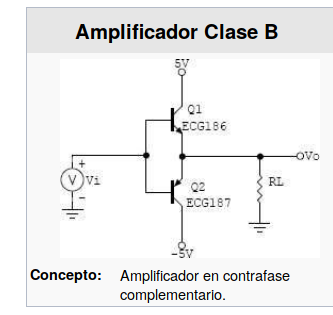
\includegraphics[scale=0.60]{ejemplo1.png}
\end{figure}
 
\begin{figure}[hbtp]
\centering
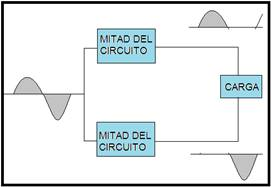
\includegraphics[scale=0.90]{ejemplo2.png}
\end{figure}

\begin{figure}[hbtp]
\centering
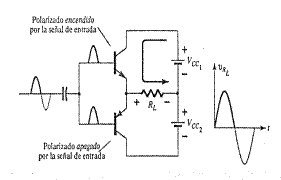
\includegraphics[scale=0.90]{ejemplo3.png}
\end{figure}   

\footnote{Universidad Politécnica De La Zona Metropolitana De Guadalajara} 
\newpage

\section{Características}

Se les denomina amplificador clase B, cuando el voltaje de polarización y la máxima amplitud de la señal entrante poseen valores que hacen que la corriente de salida circule durante el semiciclo de la señal de entrada.

La característica principal de este tipo de amplificadores es el alto factor de amplificación.

Amplificadores clase AB: Estos básicamente son la mezcla de los dos anteriores. Cuando el voltaje de polarización y la máxima amplitud de la señal entrante poseen valores que hacen que la corriente de salida circule durante menos del ciclo completo y más de la mitad del ciclo de la señal de entrada, se les denomina: Amplificadores de potencia clase AB.

Dado que ocupa un lugar intermedio entre los de clase A y AB, cuando el voltaje de la señal es moderado funciona como uno de clase A, cuando la señal es fuerte se desempeña como uno de clase B, con una eficiencia y deformación moderadas. 

\subsection{Ventajas}

\begin{itemize}


\item Posee bajo consumo en reposo.    
\item Aprovecha al máximo la Corriente entregada por la fuente.
\item Intensidad casi nula cuando está en reposo.

\end{itemize}


\subsection{Desventajas}

\begin{itemize}


\item Producen armónicos, y es mayor cuando no tienen los transistores de salida con las mismas características técnicas, debido a esto se les suele polarizar de forma que se les introduce una pequeña polarización directa. Con esto se consigue desplazar las curvas y se disminuye dicha distorsión.

\end{itemize}

\section{Aplicaciones}

\begin{itemize}
\item     Sistemas telefónicos,
    Transmisores de seguridad portátiles
    Sistemas de aviso, aunque no en audio.
\end{itemize}

\bibliography{Referencia}
\begin{thebibliography}{X}
\bibitem{Baz} \textsc{BOYLESTAD NASHELSKY.} \textit{Electronica teoría de circuitos y dispositivos electrónicos.} Editorial Perason, 8va edición, Pag 761,769.

\bibitem{Baz} \textsc{ALBERT MALVINO.} \textit{Principios de electrónica.} 
Editorial Mc Graw Hill, 6ta edición, Pag 295.


\bibitem{Baz} \textsc{Articulo:} \textit{www.metecnologico.com} 
Amplificadores Clase B.

\end{thebibliography}

\bibliographystyle{plain}

\footnote{Universidad Politécnica De La Zona Metropolitana De Guadalajara} 
\newpage

\end{document}





